\documentclass{article}

\usepackage{tikz}
\usepackage{parskip}
\usepackage{amssymb}
\usepackage[utf8]{inputenc}
\usepackage{amsmath, empheq}
\usepackage[margin=3.75cm]{geometry}
\definecolor{mycolour}{RGB}{46,52,64}
\pagecolor{mycolour}
\color{white}

\title{\jobname}
\author{Eugenio Animali}

\begin{document}
\maketitle
\section*{Equazioni importanti}
\begin{gather}
    \begin{cases}
        F=I\vec{L}\times\vec{B}\\
        F=q\vec{v}\times\vec{B}
    \end{cases}\\
    B=\frac{\mu_0}{2\pi}\frac{I}{r}
\end{gather}
\section*{Sappiamo giá}

Le linee di campo vanno da N a S e sono tutte ininterrotte.

\section*{Forza di coulomb}

La forza di coulomb é la forza che subisce una particella carica in un campo elettrico

\begin{gather*}
    \vec{F} = q\vec{E}
\end{gather*}
\section*{Forza di lorentz}
La forza di lorentz é la forza che subisce una particella carica in un campo magnetico.

Una carica é sottoposta ad un campo magnetico solo quando é in movimento.

Per $B = $ Campo magnetico, $q=$ carica della particella, e $\vec{v}=$ velocitá della particella.
\[
    \vec{F}=q\vec{v}\times\vec{B}
    \]
di cui il valore é:

    \[
    F=|q|vB\sin\alpha
\]

\begin{gather*}
    B=\frac{F}{|q|v\sin\alpha}\\
    \text{misurato in Tesla: } T=\frac{N}{C\frac{m}{s}} = \frac{N}{Am}
\end{gather*}
Questa forza non fa lavoro perche agisce perpendicolarmente allo spostamento.

Vera Forza di Lorentz:

Forza applicata su un filo elettrico in un campo magnetico.
\[\vec{F}_L=I\vec{L}\times \vec{B}\]
perché $I=\frac{q}{s}$ e $\vec{L}=v\cdot s$
\section*{Notazioni}
Un vettore che viene verso di noi é disegnato come cerchio con un punto al centro; un vettore che si allontana é disegnato come un cerchio con una x.

La regola della mano destra:

Pollice: velocitá particella

Indice: campo magnetico
\section*{Possibili traiettorie di una carica in un campo magnetico}
\begin{enumerate}

\item $\vec{v}\parallel \vec{B}$ Moto Rettilineo Uniforme
\item $\vec{v}\perp \vec{B} $ Moto circolare uniforme
\begin{gather*}
\vec{F} = q\vec{v}\times \vec{B}\\
\vec{a}_{centripeta}=\frac{\vec{F}}{m}\\
\vec{a}_{centripeta}=\frac{v^2}{r}\\
qvB=m\frac{v^2}{r}\\
qB=m\frac{v}{r}
\end{gather*}
\item Una combinazione di 1 e 2: Moto elicoidale- ha un moto circolare nella componente perpendicolare, mentre si sposta in moto rettilineo uniforme sull'asse di $\vec{B}$
\end{enumerate}
\section*{Come misurare la massa}
Mass spectrometer, possibilmente di Thompson?
\begin{enumerate}

\item Selettore di Velocitá\\
Sparo un elettrone in uno spazio con campo Magnetico (creato da magnete a ferro di cavallo) e un campo elettrico (creato da un condensatore) perpendicolari. Quando passa l'elettrone, sará spinto da due forze parallele e opposte. Cambiando le forze, posso raggiungere un equilibrio, per cui l'elettrone va dritto, allorquando so che sono uguali le due forze.
\begin{gather*}
    F_e=F_m\\
    qE=qvB\\
    E=vB
\end{gather*}
\item Spettrometro di Massa\\
L'elettrone entra in un foro; agisce su di esso un campo magnetico che lo fa girare di $180\deg$, e si schianta su uno schermo fotosensibile. Misurando la distanza dal punto illuminato sullo schermo al foro, si trova il raggio del moto circolare uniforme.

\end{enumerate}
\section*{Ciclotrone}
Condensatore permeabile con campo elettrico orizzontale in un campo magnetico verticale. L'elettrone si schianta su una parete del condensatore, entra, ruota subendo solo la forza di lorentz,quando l'elettrone ripermea l'armatura, il condensatore cambia polaritá e l'elettrone accelera verso l'altra armatura del condensatore. Cosí ripete per accelerare l'elettrone a velocitá altissime.
\section*{Motore Elettrico}
Poniamo un circuito rettangolare in un campo magnetico. Il momento di ciascun braccio $\perp$ del circuito rispetto al campo, é $\vec{F}\cdot \vec{s}$. Sappiamo che $F=I\vec{L}\times \vec{B}$. Quindi il momento di ciascun braccio, per $b=$ la distanza tra le due braccia, é $M=\frac{1}{2}b\cdot F_1$. Essendo uguali le braccia, il momento totale é $M=b\cdot F=bIhB=AIB$ per $A=$ l'area del circuito. Posso amplificare l'effetto facendo piú giri del filo per aumentare il numero di avvolgimenti, $N$: $M=NIAB$. Questa forza agisce perpendicolarmente al campo, quindi ad un certo punto inizierá a frenare il moto del circuito, dopo mezzo giro. Allora per cambiare il verso della forza dobbiamo cambiare il verso della corrente. La spira ruota, e le spazzole cambiano il contatto e scambiano anello, cambiando il verso della corrente nella spira.
\section{Circuitazione}
La circuitazione é la somma dei prodotti scalari tra una lunghezza e il campo elettrico in quel punto. $\Gamma_c=\Sigma \vec{E}\cdot \vec{\Delta l}$. In un campo elettrico uniforme, questa somme uguale 0.

Oersted scopre che un filo percorso da corrente genera un campo magnetico.

Ampere studia i campi magnetici e studia questa relazione tra circuitazione e correnti concatenate:
\begin{gather*}
     \Gamma_c(\vec{B})=\mu_0\Sigma I_{conc}\\
     \mu_0 = 4\pi \cdot 10^{-7}\frac{Tm}{A}\text{ Permeabilitá Magnetica nel vuoto}\\
     I_{conc} = \Sigma I \text{ interne alla concatenazione}\\  \text{Positive quelle che obbediscono alla regola della mano destra.}
\end{gather*}
Legge di Biot-Savart
Equazione per trovare campo magnetico causato da un filo.
\begin{gather*}
    B=\frac{\mu_0}{2\pi}\frac{I}{r}
\end{gather*}
\section*{Biot-Savart}
\subsection*{2 Fili paralleli}
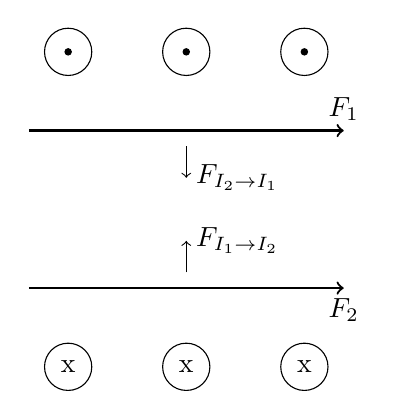
\begin{tikzpicture}
    \draw[thick,->] (-2,1) -- (2,1) node[anchor=south] {$F_1$};
    \draw[thick,->] (-2,-1) -- (2,-1) node[anchor=north] {$F_2$};
    \draw[->] (0,0.8) -- (0,0.4) node[anchor=west] {$F_{I_2 \to I_1}$};
    \draw[->] (0,-0.8) -- (0,-0.4) node[anchor=west] {$F_{I_1 \to I_2}$};
    \draw (-1.5,2) circle (0.3);
    \filldraw (-1.5,2) circle (0.04);
    \draw (0,2) circle (0.3);
    \filldraw (0,2) circle (0.04);
    \draw (1.5,2) circle (0.3);
    \filldraw (1.5,2) circle (0.04);
    \draw (-1.5,-2) circle (0.3) node {x};
    \draw (0,-2) circle (0.3) node {x};
    \draw (1.5,-2) circle (0.3) node {x};
\end{tikzpicture}

Due fili paralleli percorsi da corrente nello stesso verso si attirano.

\subsection*{Campo Magnetico di una spira di corrente}
Come un magnete -- ecco l'elettromangnete!
\section{Campi Magnetici generati da corrente}
\begin{enumerate}
    \item Filo rettilineo
    \[ B= \frac{\mu_0}{2\pi}\frac{I}{r}\]
    \item spira circolare
    \[ B_0= \frac{\mu_0}{2}\frac{I}{r}\]
    \item solenoide
    
    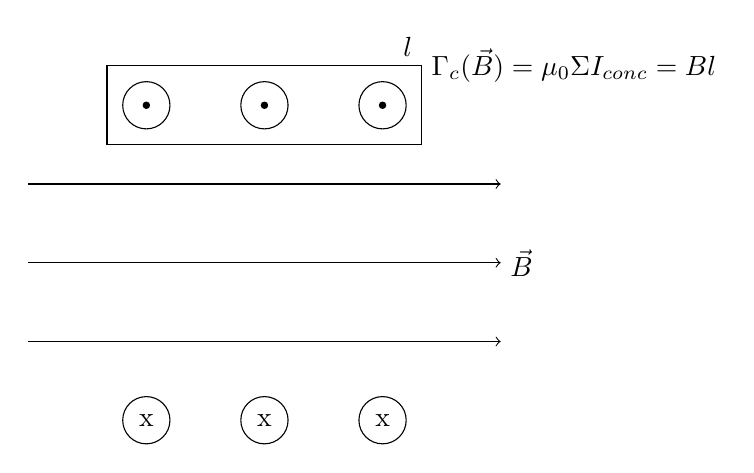
\begin{tikzpicture}
        \draw[->] (-3,1) -- (3,1);
        \draw[->] (-3,0) -- (3,0) node[anchor=west] {$\vec{B}$};
        \draw[->] (-3,-1) -- (3,-1);
        \draw (-1.5,2) circle (0.3);
        \filldraw (-1.5,2) circle (0.04);
        \draw (0,2) circle (0.3);
        \filldraw (0,2) circle (0.04);
        \draw (1.5,2) circle (0.3);
        \filldraw (1.5,2) circle (0.04);
        \draw (-1.5,-2) circle (0.3) node {x};
        \draw (0,-2) circle (0.3) node {x};
        \draw (1.5,-2) circle (0.3) node {x};
        \draw (-2,1.5) rectangle (2,2.5) node[anchor=west] {$\Gamma_c(\vec{B})=\mu_0\Sigma I_{conc}=Bl$} node[anchor=south east] {$l$};
    \end{tikzpicture}
\end{enumerate}
\section{Permeabilitá magnetica di un materiale}
\[\frac{B}{B_0}=\mu_r\]
\begin{enumerate}
    \item se $\mu_r \gg 1$: (es. 100000) Ferromagnetico
    \item se $\mu_r > 1$: (es. 1,0004) Paramagnetico
    \item se $\mu_r < 1$: (es. 9,9993) Diamagnetico
\end{enumerate}
\section{Induzione Elettromagnetica}
\subsection{storia}
Faraday prende una sbarra di ferro e ci avvolge due circuiti sulle due estremitá. Il primo ha un generatore e il secondo ha un amperometro ma non c'é un generatore. al momento dell'accensione del generatore, si vede passare corrente nell'amperometro, che poi si riduce subito a nulla.

Se faccio passare un magnete dentro alla spira con l'amperometro, passa corrente.
\subsection{Flusso del Campo Magnetico}
\begin{gather*}
\Phi(\vec{B})=\vec{B}\times\vec{S}=BS\cos \theta\\
\Phi_{\perp}(\vec{B})=BS\\
\Phi_{\parallel}(\vec{B})=0
\end{gather*}
\subsection{Legge di Faraday-Neumann-Lenz}
\[fem_i=-N\frac{\Delta\Phi(\vec{B})}{\Delta t}\]

Per fare corrente serve un $\Delta\Phi(\vec{B})$, che puó essere causato da un $\Delta$ nel Campo, la superficie interna alla spira, o la direzione del filo.

La N rappresenta il numero di spire.

Il verso é negativo perché l'elettricitá generata deve creare un campo che oppone quello che la ha generata.
\section{Fem indotta in Generatore}
Da imparare a memoria
\begin{gather*}
    \alpha = \omega t\\
    \Phi = BS\cos \alpha\\
    \Phi = BS\cos \omega t\\
fem = -N\frac{d\Phi}{dt} = +NBS\omega\sin(\omega t)
\end{gather*}
\subsection{Circuito Autoinducente, Circuito RL in CC}
solenoide in circuito. quando si chiude il circuito, varia campo magnetico $B= \mu_0 \frac{N}{l}I$ che fa variare il flusso. Per la legge di Lenz si deve creare una forza opposta, che rallenta la corrente, rendendo piú lento il processo di raggiungere l'equilibrio.
\begin{gather*}
I = \frac{E}{R}(1 - e^{-\frac{t}{\tau}})
\end{gather*}
\subsection{L di Henry}
L é l'induttanza
\begin{gather*}
    L= \mu_0\frac{N^2}{l}S
\end{gather*}
\section{}
pg.49
\begin{gather*}
    U=\frac{1}{2}LI^2
\end{gather*}
\section{Trasformatori}

Due circuiti avvolti attorno a due lati di un toro. Uno fornisce la tensione, l'altro la induce attraverso il toro.

\begin{gather*}
    \mathcal{E}_1=N_1\frac{\Delta\Phi}{\Delta t}\\
    \mathcal{E}_2=N_2\frac{\Delta\Phi}{\Delta t}\\
    \frac{\mathcal{E}_1}{\mathcal{E}_2}=\frac{N_1}{N_2}\\
    P=IV\\
    \frac{\mathcal{E}_1}{\mathcal{E}_2}=\frac{N_1}{N_2}=\frac{I_2}{I_1}\\
\end{gather*}
\section{Circuiti in Corrente Alternata}
\begin{gather*}
    V(t)=V_{max}\sin (\omega t)\\
    V(t)=RI(t)\\
    I(t)=I_{max}\sin (\omega t)\\
    V_{max}=I_{max}
\end{gather*}
\subsection{Piano dei Fasori}
Si puó immaginare i vettori $I_{max}$ e $V_{max}$ che ruotano attorno all'origine del piano cartesiano, e $I$ e $V$ valgono il seno di queste, o la loro proiezione su qualsiasi retta passante per l'origine. Non mi importa il valore in tempo $t$ ma il relativo valore tra $I$ e $V$.

\subsection{Media quadratica}
\begin{gather*}
    \sqrt{\frac{I_{max}^2}{2}}=\frac{I_{max}}{\sqrt{2}}
\end{gather*}
\section{Circuito puramente resistivo R in CA}
\begin{gather*}
    I(t) = I_{max}\sin \omega t\\
    V(t) = V_{max}\sin \omega t\\
    P(t)=V(t)\cdot I(t)=V_{m}I_m\sin^2 \omega t\\
    \overline{P}=\frac{V_mI_m}{2}=V_{eff}\cdot I_{eff}
\end{gather*}
\section{Circuito C in CA}
\begin{gather*}
    V(t)=V_m\sin \omega t\\
    Q=CV\\
    Q(t)=CV_m\sin \omega t\\
    I(t)=\frac{dQ}{dt}\\
    I(t)=\omega \cdot CV_m\cos \omega t\\
    I(t)=\underbrace{\omega CV_m}\cos \omega t\\
    I_m\\
    P=VI=\\
    V_mI_m\sin \omega t \cos \omega t=\\
    \frac{1}{2}V_mI_m\sin (2\omega t)
\end{gather*}
\section{Circuito L in CA}
\section{4 regole di maxwell}
\begin{enumerate}
    \item Flusso di $\vec{E}$
    (Legge di Gaus)
    \begin{gather*}
        \Phi_c(\vec{E})=\frac{\sum Q_{int}}{\epsilon}
    \end{gather*}
    \item Flusso di $\vec{B}$
    \begin{gather*}
    \Phi_c(\vec{B})=0
    \end{gather*}
    \item Circuitazione di $\vec{E}$
    (Legge di Faraday-Neumann-Lenz)
    \begin{gather*}
        \Gamma_c(\vec{E})=\Sigma\vec{E}_i\Delta\vec{l}_i\\
        \Gamma_c(\vec{E})=-\frac{d\Phi(\vec{B})}{dt}
    \end{gather*}
    \item Circuitazione di $\vec{B}$
    (Legge di Ampere-Maxwell)
    \begin{gather*}
        \Gamma_c(\vec{B})=\mu_0\epsilon_0\frac{d\Phi(\vec{E})}{dt}
    \end{gather*}
\end{enumerate}
\section{Corrente di Spostamento}
In un condensatore, non passano cariche, ma c'é una certa quantitá di campo magnetico lá in mezzo. Quindi passa qualcosa che non é propriamente una corrente ma ha le stesse unitá di misura. si chiama corrente di spostamento.
\begin{gather*}
    I_s=\varepsilon_0\frac{d\Phi(\vec{E})}{dt}
\end{gather*}
\section*{equazione dell'onda}
\begin{gather*}
    \vec{E}=E_{max}\cos[\omega t-kx]\hat{j}\\
    \vec{B}=B_{max}\cos[\omega t-kx]\hat{k}\\
    k=\text{numero d'onda}=\frac{2\pi}{\lambda}\\
    \omega=\frac{2\pi}{T}\\
\end{gather*}
\section{Vettore di Poynting}
\begin{gather*}
    \vec{S}=\frac{1}{\mu_0}\vec{E}\times\vec{B}
\end{gather*}
\end{document}